\section{実験}
\label{sec:実験}
\subsection{把持実験}
本グリッパの指を入れ替えて対象物の把持の可不可を検証する.指の種類はゲル,バネ,ゴムで被覆したスポンジ,柔軟物なしのものとし以下にまとめる.検証に用いる把持対象物を\refig{denso_parts}に示す.把持対象物は自動車部品工場で用いられる部品のモデルの5種類とし,それぞれA,B,C,D,Eの記号を部品ごとに割り振った.
また,把持対象物Eは\refig{E}上部の突起部と下部の外周部でそれぞれ把持実験を行った.



\subsubsection{実験手順}

\begin{enumerate}
  \item 上記の把持対象物を作業台に配置した.  
  \item グリッパの指を開き作業台の鉛直上方向から把持に適切な位置まで接近させた. 
  \item グリッパの指を閉じ把持対象物を把持した.
  \item 把持対象物を把持したまま鉛直上方向に持ち上げることができれば把持可能,持ち上げることができなければ把持不可能と判別した.
\end{enumerate}

\begin{figure}[h]
 \begin{center}
  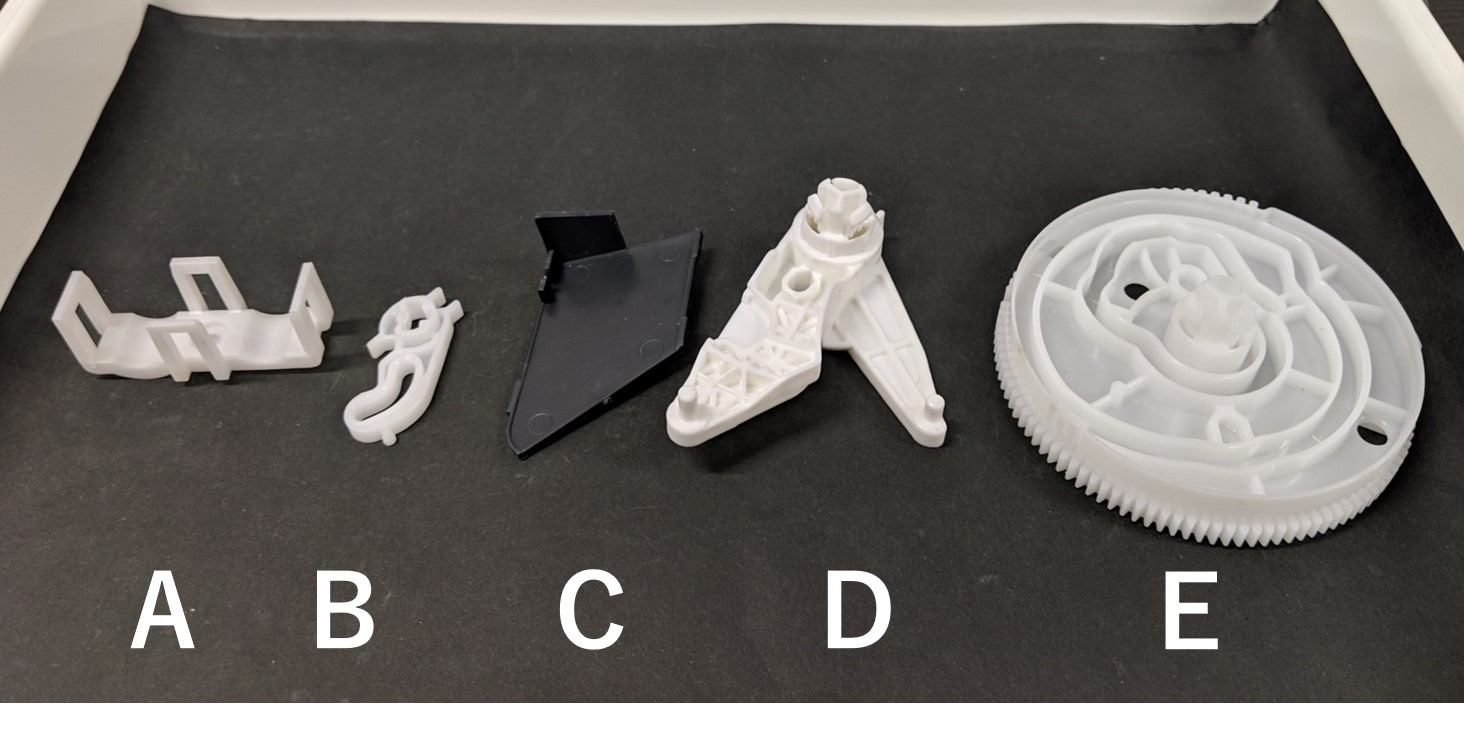
\includegraphics[scale=0.6]{../figure/denso.eps}
 \caption{自動車部品}
  \label{fig::denso_parts}
 \end{center}
\end{figure}

\begin{figure}[h]
 \begin{center}
  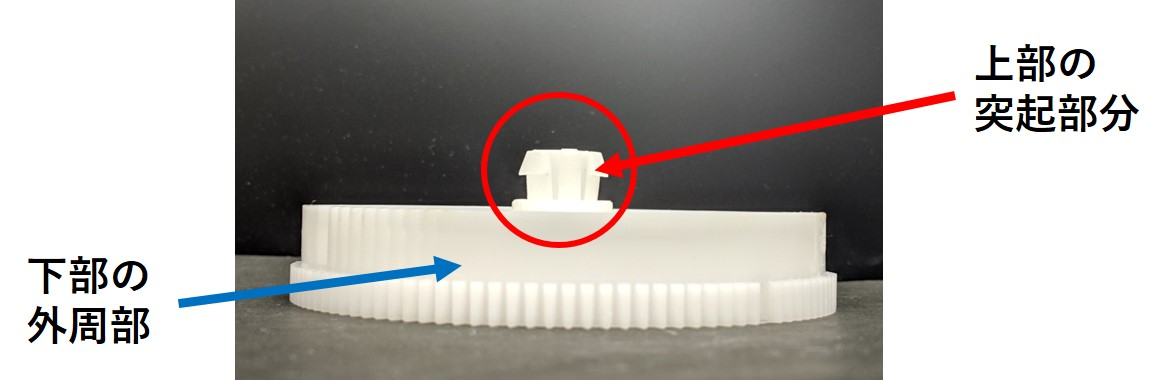
\includegraphics[scale=0.6]{../figure/E.eps}
 \caption{把持対象物E}
  \label{fig::E}
 \end{center}
\end{figure}

\newpage


\subsubsection{実験結果}
使用した指は以下の通りである.実験結果を\reftab{result}にまとめる.把持成功は◯,把持失敗は×を表している.把持対象物Eは上部の突起部と下部の外周部での把持が両方成功した時把持成功とみなした.\reftab{result}の横軸は\refig{denso_parts}の割り振った記号と対応し縦軸は以下の指の番号と対応している.

\begin{enumerate}
  \item 柔軟物のない指
  \item 厚さ3mmのゲルを取り付けた指
  \item 厚さ6mmのゲルを取り付けた指
  \item 厚さ9mmのゲルを取り付けた指
  \item 厚さ6mmのゴムで覆ったスポンジを取り付け指
  \item 厚さ8mmのゴムで覆ったスポンジを取り付け指
  \item 厚さ10mmのゴムで覆ったスポンジを取り付け指
  \item 内径6mmのばねを取り付けた指
  \item 内径7mmのばねを取り付けた指
  
\end{enumerate}

\begin{table}[htbp]
    \caption{把持実験結果}
   \label{tab::result}
   %\scalebox{3}[1.5]
   \centering
   \begin{tabular}{|c||c|c|c|c|c|} \hline
          &A    &B     &C      &D     &E        \\ \hline \hline
        (1) & ◯ & ◯  & ×  & ◯ & ×  \\ \hline
        (2) & ◯ & ◯  & ◯  & ◯ & ◯  \\ \hline
        (3) & ◯ & ◯  & ◯  & ◯ & ◯  \\ \hline
		(4) & ◯ & ◯  & ◯  & ◯ & ×  \\ \hline
		(5) & ◯ & ◯  & ◯  & ◯ & ×  \\ \hline				
		(6) & ◯ & ◯  & ◯  & ◯ & ×  \\ \hline
		(7) & ◯ & ◯  & ◯  & ◯ & ×  \\ \hline
		(8) & × & ×  & ×  & × & ×  \\ \hline		
		(9) & × & ×  & ×  & × & ×  \\ \hline		
			
		
    \end{tabular}
\end{table}

\begin{figure}[h]
\centering
\subfloat[把持対象物A]{\includegraphics[scale=0.4]{../figure/result_a.eps}}
\hspace{5mm}
\subfloat[把持対象物B]{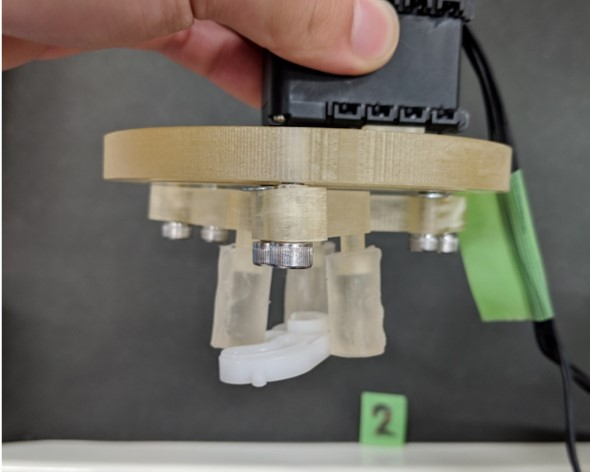
\includegraphics[scale=0.4]{../figure/result_b.eps}}
\hspace{5mm}
\subfloat[把持対象物C]{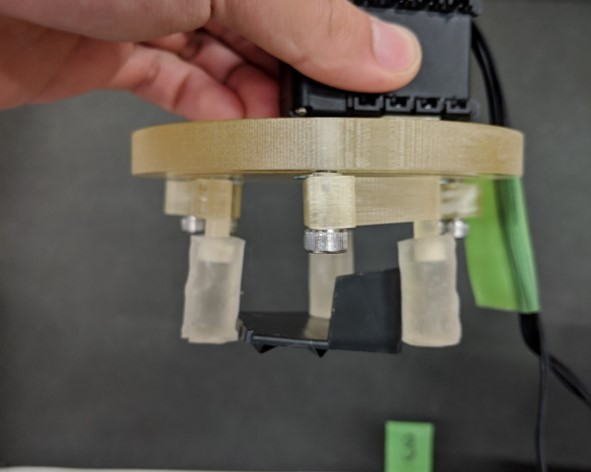
\includegraphics[scale=0.4]{../figure/result_c.eps}}
\hspace{5mm}
\subfloat[把持対象物D]{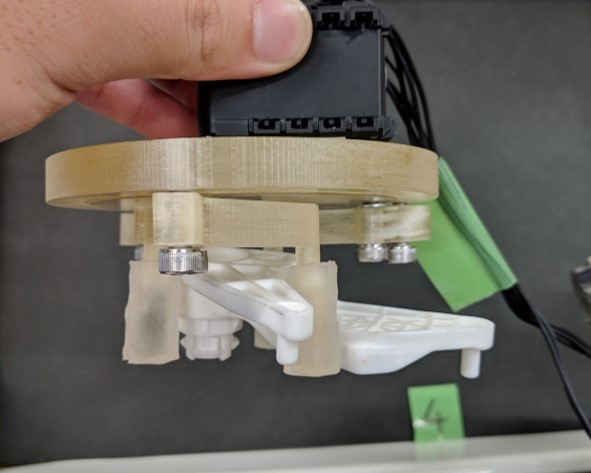
\includegraphics[scale=0.4]{../figure/result_d.eps}}
\hspace{5mm}
\subfloat[把持対象物E 上部の突起]{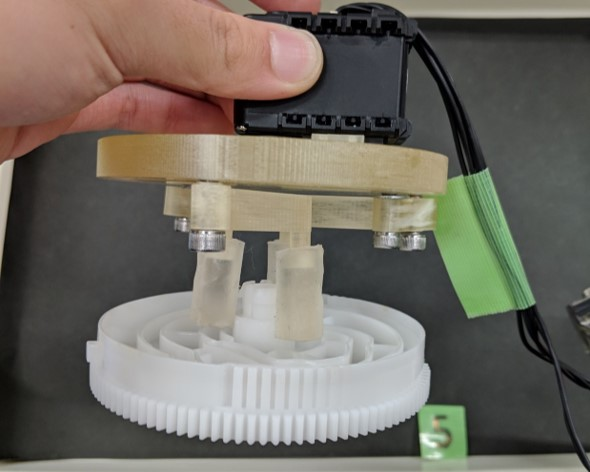
\includegraphics[scale=0.4]{../figure/result_e1.eps}}
\hspace{5mm}
\subfloat[把持対象物E 下部の外周部]{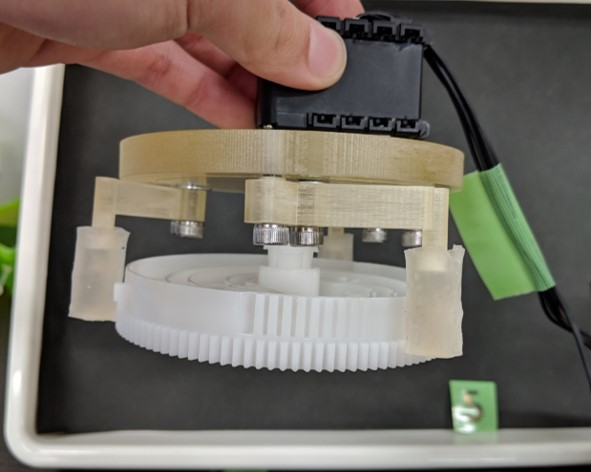
\includegraphics[scale=0.4]{../figure/result_e2.eps}}
\hspace{5mm}
\caption{厚さ3mmのゲルの指での把持の様子}
\label{fig::sisaku}
\end{figure}


